\begin{figure}[!t]
\centering
%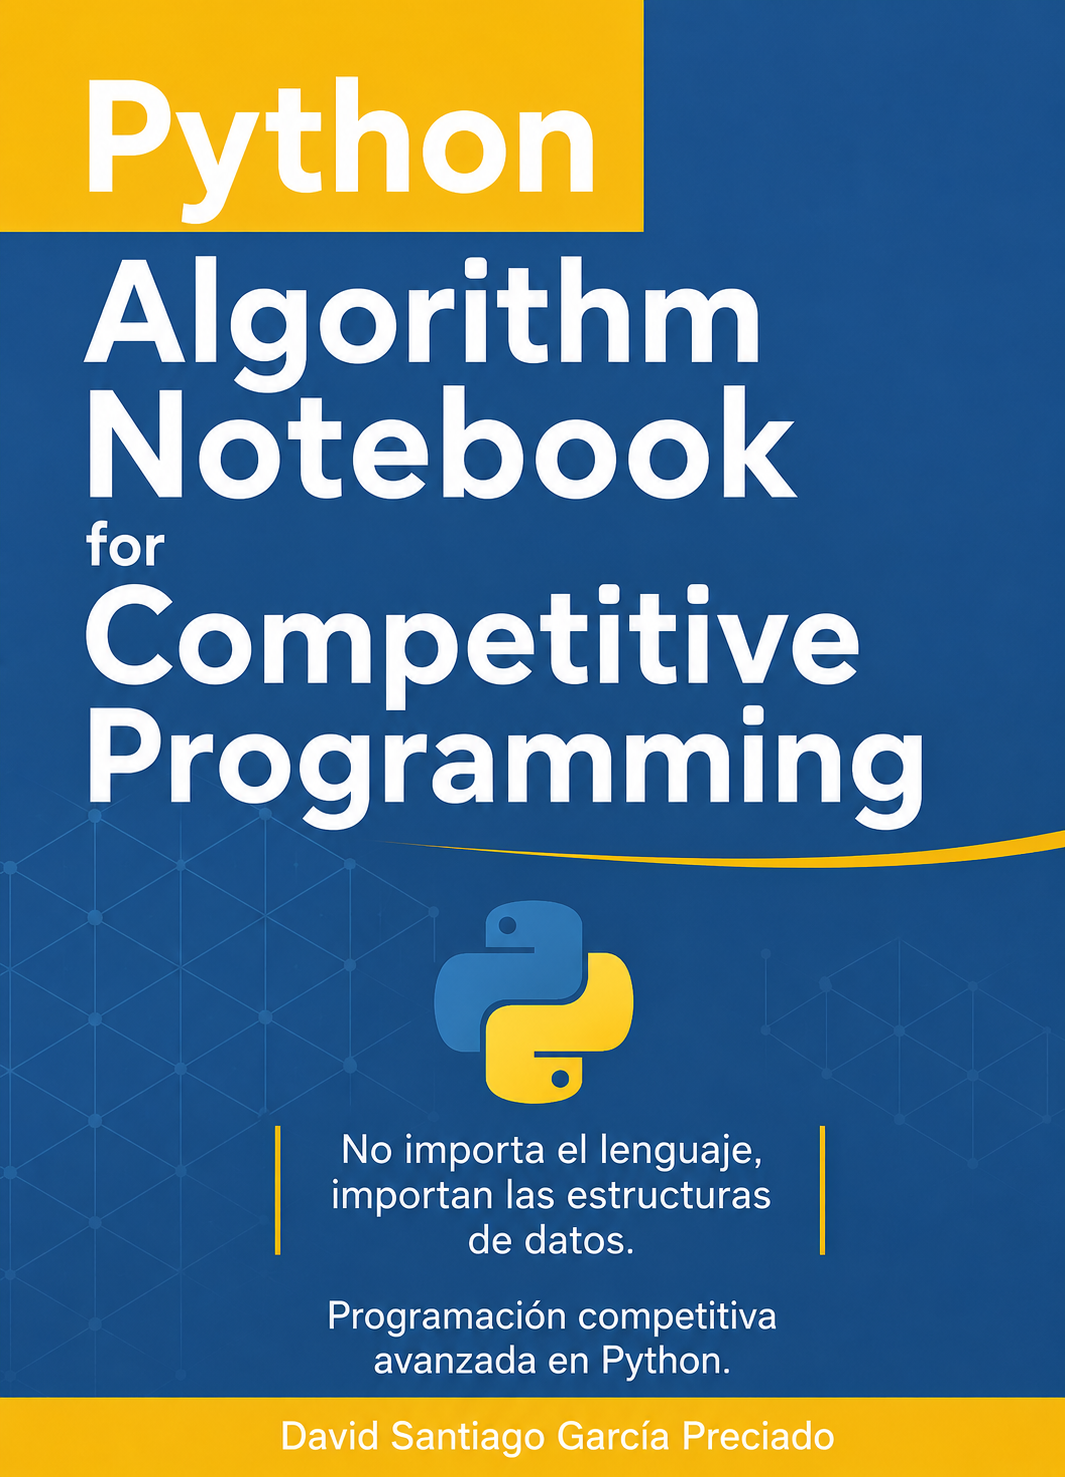
\includegraphics[width=\linewidth]{images/image1.png}
\end{figure}

Cada entrada de este cuaderno sigue siempre la misma estructura: preguntas guía para reconocer cuándo aplica el algoritmo en el contrarreloj, para qué sirve, su complejidad, el fundamento teórico, una plantilla genérica en Python comentada, y un ejercicio real resuelto con esa técnica. Este es un documento vivo: se irá ampliando problema a problema a medida que se resuelvan más ejercicios de cara a la Clasificatoria Nacional ICPC Colombia 2026.
